\chapter{Évaluation des modèles et résultats}

\section{Objectif et organisation de l'évaluation}

Ce chapitre évalue la capacité du système à reconnaître douze gloses LSFB isolées à partir de landmarks. L'objectif n'est pas de mesurer une traduction ouverte de phrases, mais de comparer des représentations et des classifieurs dans un protocole contrôlé, puis d'identifier la configuration retenue pour l'application web.

Les expériences utilisent les splits officiels de LSFB-ISOL. Les signeurs de test ne sont pas utilisés pour l'entraînement. Lorsque cela est indiqué, chaque classe est limitée à 100 séquences d'entraînement et 50 séquences de test. Les métriques principales sont l'accuracy, le macro-F1 et la balanced accuracy. Le macro-F1 est privilégié pour éviter qu'une bonne performance sur quelques classes masque des classes moins bien reconnues.

Le chapitre distingue les performances du classifieur et les contrôles d'intégration. Les détails du contrat HTTP et des endpoints sont définis dans le chapitre consacré à l'application ; ici, le test d'intégration est utilisé uniquement pour vérifier que le modèle gelé est reproduit sans modification lors du déploiement.

\section{Protocole scientifique et gel de la configuration GRU retenue}

Le protocole final a été gelé avant la comparaison du test officiel. Il utilise le vocabulaire contrôlé de douze gloses, les 7\,590 séquences d'entraînement autorisées et les 5\,957 séquences du test officiel. La séparation est faite par signeur : les 59 signeurs d'entraînement et les 40 signeurs de test ne se recouvrent pas. Les doublons d'identifiants et les doublons de lignes sont contrôlés avant l'entraînement.

La validation interne utilise trois graines, 7, 42 et 101, et cinq folds stratifiés groupés par signeur. Chaque checkpoint est sélectionné uniquement sur la validation de son fold avec le macro-F1. Les données de validation ne sont pas mélangées avec les données d'entraînement et le test officiel n'est pas utilisé pour régler les hyperparamètres, les représentations ou l'arrêt précoce.

La configuration GRU retenue reprend le protocole d'GRU initiale et ajoute uniquement les deux poignets relatifs au centre des épaules. Les autres éléments sont conservés : corpus, classes, graines, folds, longueur de 32 frames, architecture GRU et règle d'optimisation. Cette contrainte permet d'interpréter l'expérience comme une ablation ciblée de la représentation, même si la comparaison finale avec le RF reste une comparaison de configurations complètes.

Le modèle est gelé pour trois raisons. Premièrement, configuration GRU retenue obtient le meilleur macro-F1 de validation moyen parmi les configurations GRU comparées, avec 0,7326 et un écart-type de 0,0309. Deuxièmement, il améliore le résultat de test d'GRU initiale, de 0,8130 à 0,8153 en macro-F1, avec une balanced accuracy de 0,8129. Troisièmement, les quinze checkpoints, leurs manifestes et les tests API sont archivés et reproduisent le contrat d'inférence. Le gain est faible ; le gel ne signifie donc pas que la supériorité est définitivement prouvée. Il signifie que la configuration est figée pour éviter de modifier le modèle après consultation du test.

Après le gel, aucune modification de poids, de classes, de prétraitement ou de seuil de décision n'est appliquée pour améliorer le score du test officiel. Toute calibration de confiance ou politique de rejet future devra être apprise sur une validation séparée et enregistrée comme une nouvelle étape, sans réécrire les résultats de la configuration GRU retenue.

\section{Synthèse des études récentes}

Les premières expériences du projet ont servi à vérifier la faisabilité du pipeline et à comparer quelques représentations sur des sous-échantillons limités. Elles sont conservées dans les journaux expérimentaux et les annexes, mais elles ne constituent pas le résultat principal du mémoire. La suite de l'analyse porte sur les expériences récentes, conduites sur les partitions officielles et avec une validation groupée par signeur lorsque cela est possible.

\begin{table}[ht]
\centering
\small
\caption{Succession des configurations dans la stratégie champion/challenger.}
\label{tab:champion-challenger}
\begin{tabular}{p{3.2cm}p{3.3cm}p{5.0cm}p{3.8cm}}
\hline
Configuration & Représentation & Rôle dans la sélection & Statut final \\
\hline
RF plafonné & \texttt{raw}/\texttt{wrist\_scaled} & Baseline exploratoire sur corpus limité & Écarté \\
Random Forest complet & \texttt{wrist\_scaled} séquence complète & Challenger RF avec toutes les séquences d'entraînement & Référence et repli \\
GRU initiale & Pose--mains normalisées & Challenger temporel groupé par signeur & Dépassé par configuration GRU retenue \\
GRU retenue avec poignets relatifs & Pose--mains + poignets relatifs & Ablation finale et test API de robustesse & Modèle actif \\
\hline
\end{tabular}
\end{table}

Le Tableau~\ref{tab:champion-challenger} distingue les résultats exploratoires des décisions finales. Les chiffres du test officiel sont utilisés uniquement pour comparer les candidats gelés ; les représentations et les hyperparamètres sont réglés sur la validation groupée.

La Figure~\ref{fig:revision-boxplot} présente la dispersion des scores de validation des quinze folds GRU. Le Random Forest complet est affiché comme une référence ponctuelle du test verrouillé, car son artefact complet ne fournit pas une distribution de folds directement comparable à celle des GRU.

\begin{figure}[ht]
\centering
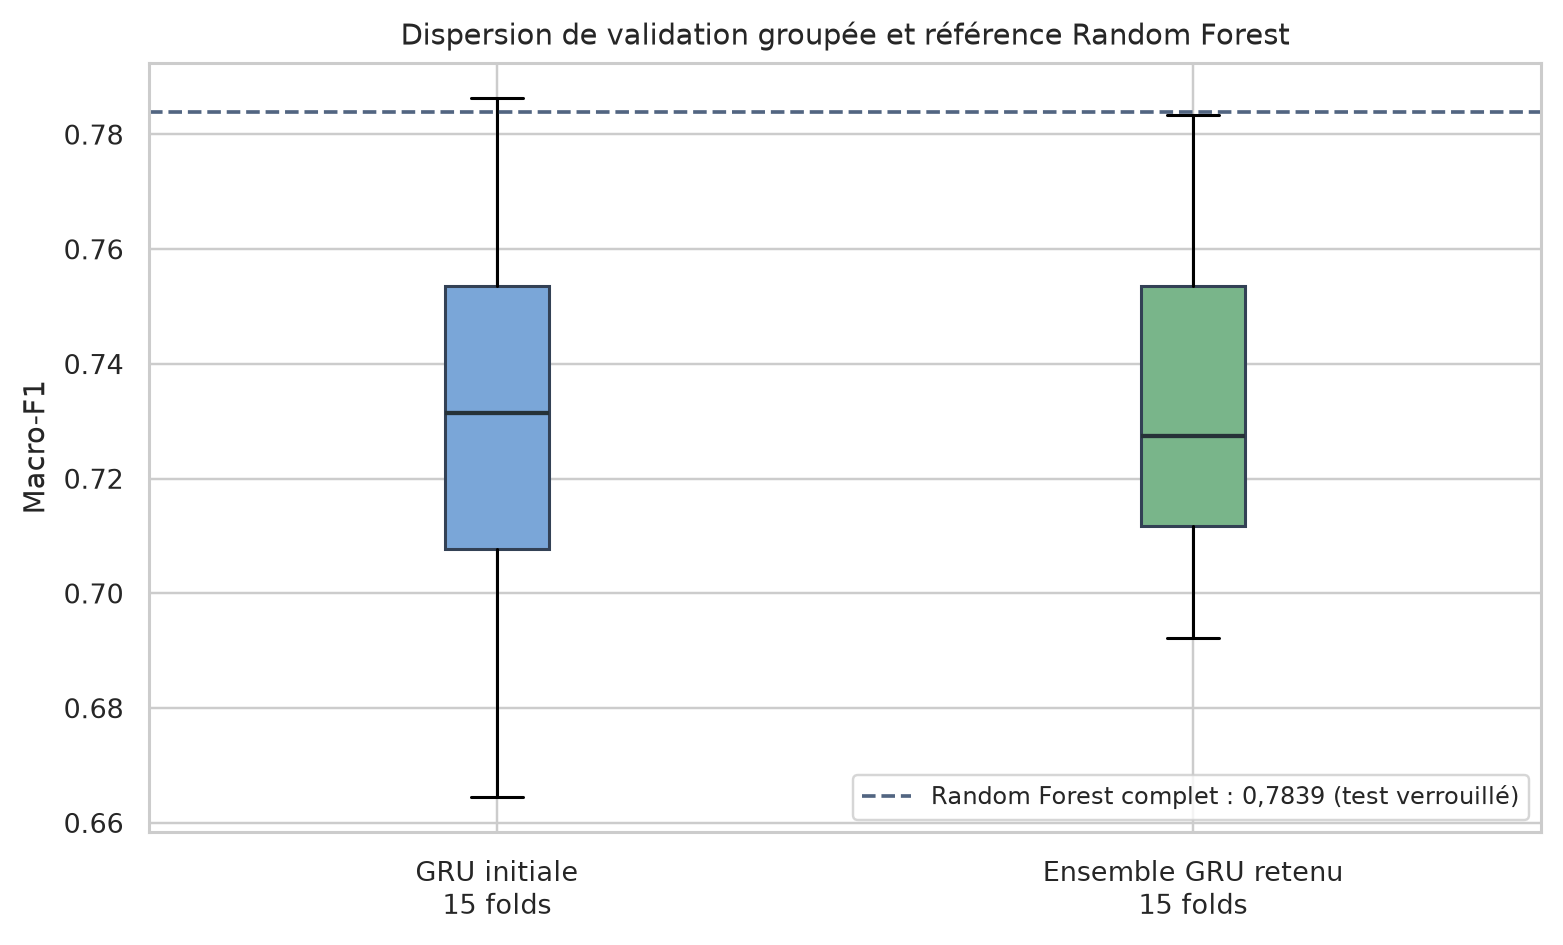
\includegraphics[width=0.94\textwidth]{figures/generated/revision_boxplot_macro_f1_gru_rf.png}
\caption{Dispersion du macro-F1 sur les folds groupés des GRU initiale et configuration GRU retenue ; la ligne pointillée indique le score de test verrouillé du Random Forest complet.}
\label{fig:revision-boxplot}
\end{figure}

\subsection{GRU initiale : validation groupée de la GRU}

GRU initiale évalue une GRU bidirectionnelle compacte avec 32 frames, trois graines (7, 42 et 101) et cinq folds groupés par signeur. Les signeurs de validation restent donc séparés des signeurs utilisés pour l'entraînement. Les quinze checkpoints atteignent un macro-F1 de validation moyen de 0,7297, avec un écart-type d'échantillon de 0,0344. Sur le test officiel verrouillé de 5\,957 séquences, l'agrégation des quinze modèles atteint une accuracy de 82,21\,%, un macro-F1 de 0,8130 et une balanced accuracy de 0,8099.

Ce résultat établit la GRU comme le meilleur candidat expérimental avant l'ablation suivante. Il doit cependant être interprété comme le résultat d'un ensemble de quinze checkpoints, et non comme la performance d'une GRU unique. La dispersion du macro-F1 par signeur reste importante : elle montre que la généralisation dépend encore des caractéristiques des signeurs et des conditions de capture.

\subsection{configuration GRU retenue : ablation des poignets relatifs au torse}

La configuration GRU retenue ajoute aux landmarks pose--mains les positions des deux poignets relatives au centre des épaules. Le corpus, les graines, les folds et les hyperparamètres restent inchangés par rapport à GRU initiale. Le macro-F1 moyen de validation progresse de 0,7297 à 0,7326, tandis que l'écart-type passe de 0,0338 à 0,0309. Sur le test officiel, l'accuracy progresse de 82,21\,% à 82,31\,%, le macro-F1 de 0,8130 à 0,8153 et la balanced accuracy de 0,8099 à 0,8129.

L'analyse par classe nuance ce gain global. Les améliorations les plus importantes concernent SOURD (+0,0258 de F1), COMPRENDRE (+0,0180), NON (+0,0166) et REGARDER (+0,0117). En revanche, BIEN (-0,0190), QUOI (-0,0130), DIRE (-0,0128) et AVOIR (-0,0125) se dégradent. La confusion NON vers SOURD diminue de 87 à 68 occurrences et la confusion FINIR vers OUI diminue de 56 à 50. À l'inverse, la confusion AVOIR vers QUOI augmente de 36 à 49 occurrences. L'ajout des poignets améliore donc certaines ambiguïtés spatiales sans résoudre toutes les confusions gestuelles.

Le gain de 0,0023 de macro-F1 sur le test est faible. configuration GRU retenue est ainsi conservée comme meilleure configuration observée, mais elle ne doit pas être présentée comme une amélioration définitivement robuste avant une réplication sur de nouvelles partitions de signeurs.

\subsection{Random Forest complet et calibration}

Le Random Forest complet réentraîne le Random Forest avec l'ensemble des 7\,590 séquences d'entraînement, au lieu du plafond historique de 100 séquences par classe. Pour permettre une comparaison correcte avec configuration GRU retenue, le protocole retenu rééchantillonne chaque séquence complète sur 32 frames, puis applique \texttt{wrist\_scaled} aux deux mains. L'entrée possède la forme \texttt{[32,126]} avant aplatissement. Le classifieur utilise 300 arbres et des poids équilibrés. Le paramètre \texttt{max\_features} vaut \texttt{sqrt}, avec une graine fixée à 42.

Sur les mêmes 5\,957 séquences de test, le RF complet atteint une accuracy de 79,03\,%, un macro-F1 de 0,7839 et une balanced accuracy de 0,7931. Il améliore donc nettement les anciennes baselines limitées, mais reste inférieur à l'ensemble GRU retenu. Le premier essai causal d'Random Forest complet, qui segmentait les séquences avant le rééchantillonnage, n'atteignait que 73,14\,% d'accuracy. Cette différence montre que la segmentation causale et la classification hors ligne ne doivent pas être confondues.

La calibration isotonic réduit l'Expected Calibration Error du RF de 0,2124 à 0,0455 et le Brier score de 0,3665 à 0,3037. Elle rend les scores plus interprétables comme niveaux de confiance, mais diminue légèrement l'accuracy de 79,03\,% à 78,73\,% et le macro-F1 de 0,7839 à 0,7801. Le modèle calibré est donc utile pour une politique de rejet, mais ne doit pas être activé uniquement pour maximiser la classification.

La Figure~\ref{fig:revision-reliability} complète ces métriques par un diagramme de fiabilité. Les courbes restent éloignées de la diagonale pour le RF brut, tandis que la calibration isotonic redistribue les niveaux de confiance. Cette figure concerne le RF. La GRU active expose désormais séparément son score brut, sa marge et l'accord des quinze réseaux, mais son artefact de température n'est pas encore produit : les scores GRU restent donc explicitement non calibrés.

\begin{figure}[ht]
\centering
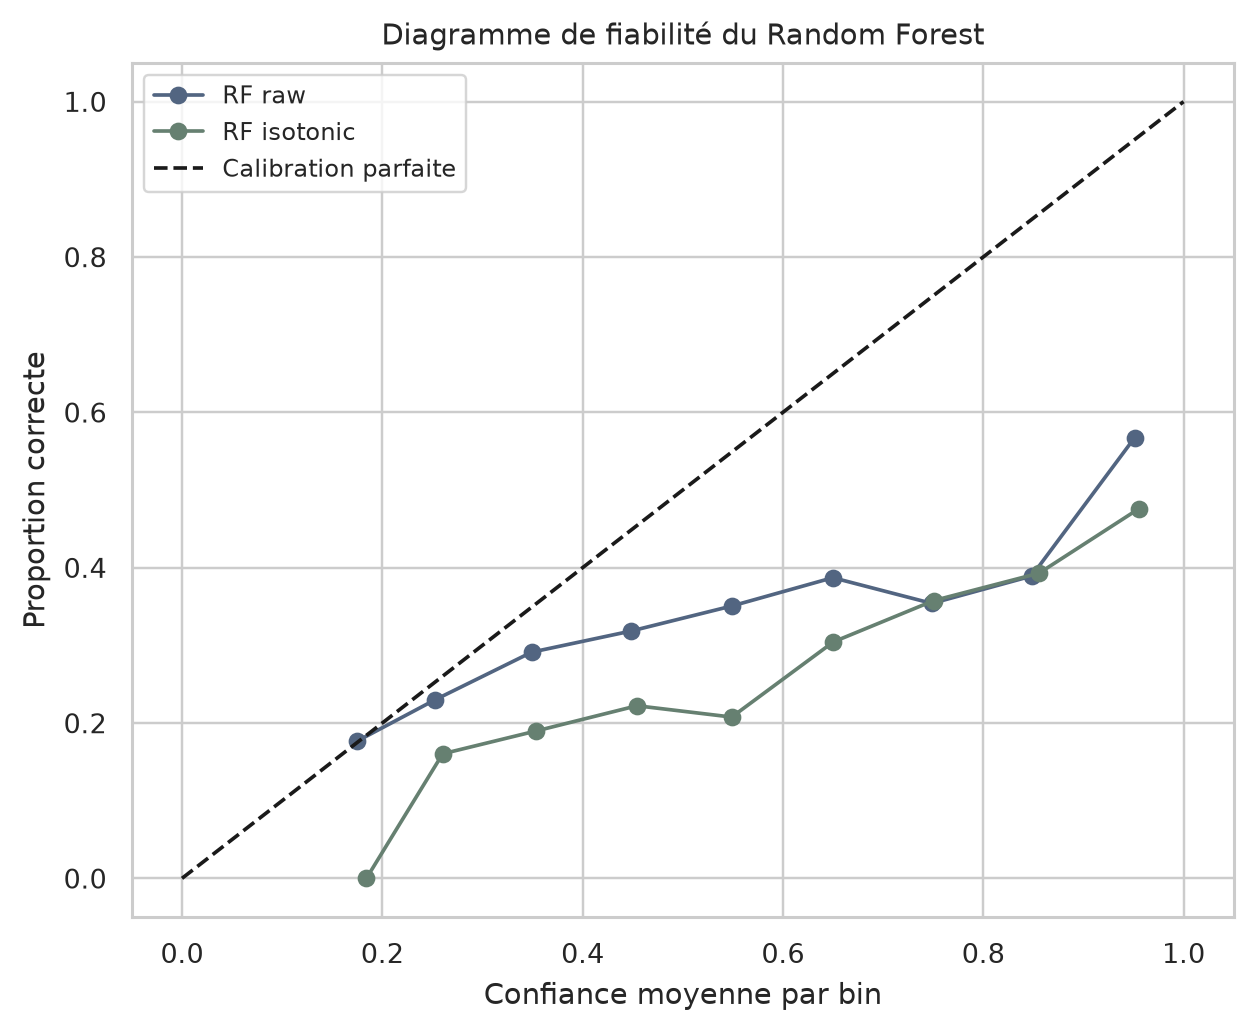
\includegraphics[width=0.90\textwidth]{figures/generated/revision_reliability_rf.png}
\caption{Diagramme de fiabilité du Random Forest complet avant et après calibration isotonic sur le test officiel.}
\label{fig:revision-reliability}
\end{figure}

\subsection{Comparaison récente et décision}

Le tableau suivant rassemble les résultats qui doivent être retenus dans la discussion du mémoire. Les anciennes expériences servent uniquement à documenter la progression du projet ; elles ne doivent pas être utilisées pour comparer directement les modèles récents, car leurs tailles de corpus, représentations et règles de fenêtrage diffèrent.

Le Tableau~\ref{tab:recent-results-summary} donne les métriques principales, et le Tableau~\ref{tab:gru-api-per-class} détaille la robustesse de l'ensemble GRU par glose.

\begin{table}[ht]
\centering
\small
\caption{Résultats récents sur le test officiel de 5\,957 séquences.}
\label{tab:recent-results-summary}
\begin{tabular}{lccc}
\hline
Configuration & Accuracy & Macro-F1 & Balanced accuracy \\
\hline
Random Forest complet & 79,03\,\% & 0,7839 & 0,7931 \\
RF calibré isotonic & 78,73\,\% & 0,7801 & 0,7853 \\
GRU initiale, 15 checkpoints & 82,21\,\% & 0,8130 & 0,8099 \\
GRU retenue avec poignets relatifs, 15 checkpoints & \textbf{82,31\,\%} & \textbf{0,8153} & \textbf{0,8129} \\
\hline
\end{tabular}
\end{table}

La Figure~\ref{fig:revision-class-bars} met en évidence les différences par glose. Le gain de la GRU n'est pas uniforme : il est particulièrement visible pour DIFFERENT, OUI et SOURD, tandis que certaines classes comme QUOI restent proches du RF et que les confusions FINIR ou NON demeurent difficiles. Les classes NON et SOURD sont surlignées, car leur séparation reste un point de diagnostic important.

\begin{figure}[ht]
\centering
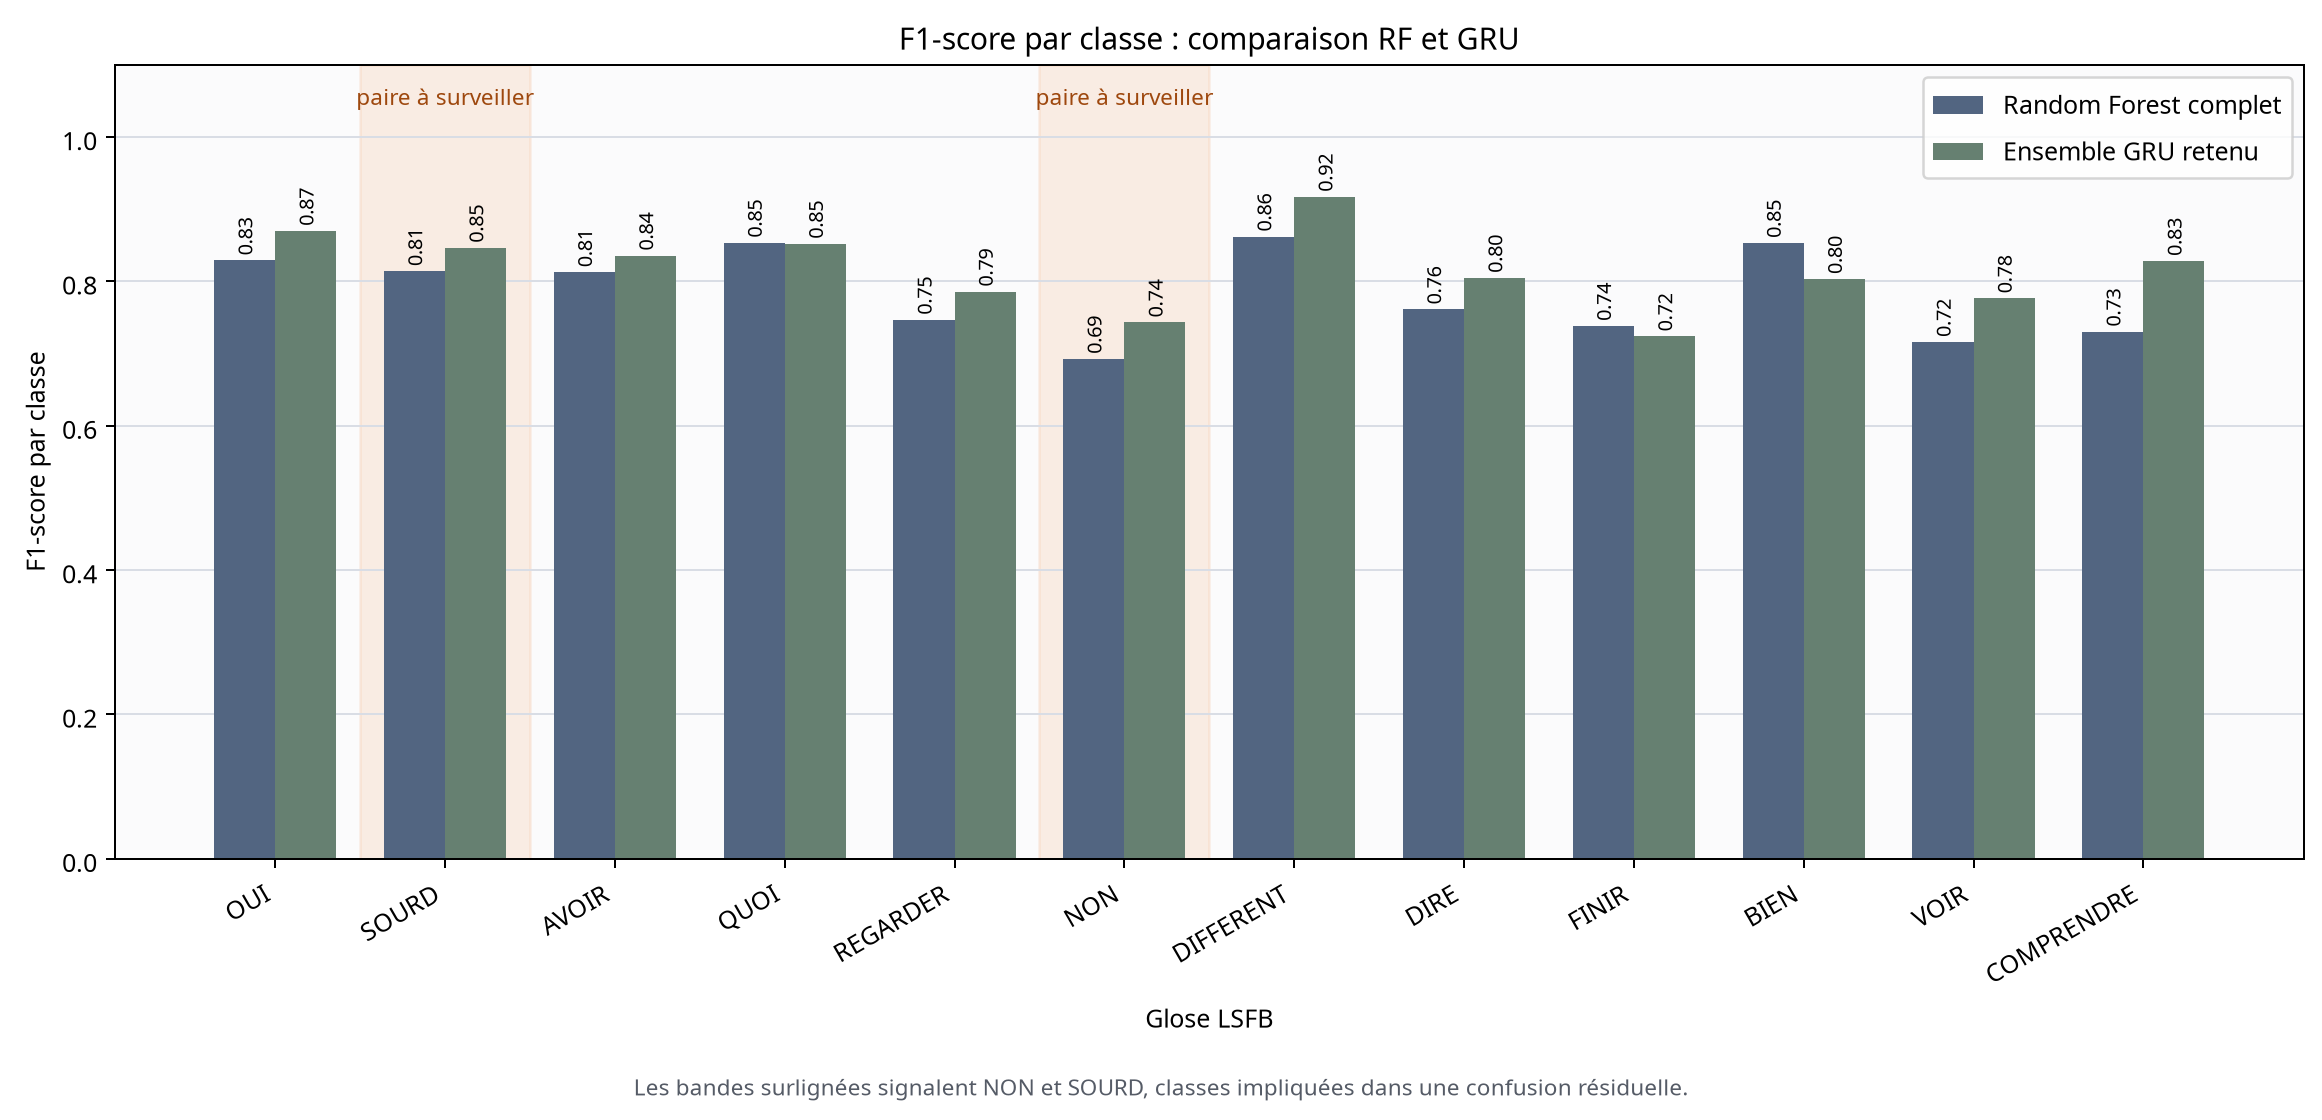
\includegraphics[width=0.98\textwidth]{figures/generated/f1_par_classe_gru_rf_non_sourd.png}
\caption{F1-score par classe entre le Random Forest complet et l'ensemble GRU retenu sur le test officiel. Les bandes indiquent NON et SOURD.}
\label{fig:revision-class-bars}
\end{figure}

L'ensemble GRU retenu constitue le meilleur résultat expérimental observé et devient également le modèle actif de l'application. Le RF complet reste conservé pour les comparaisons et le retour arrière. Cette décision est fondée sur le gain mesuré sur le test officiel et sur la vérification du contrat d'inférence, tout en conservant une surveillance de la latence.

\subsection{Pistes d'amélioration fondées sur les résultats récents}

La prochaine amélioration prioritaire consiste à comparer RF et GRU avec la même représentation, les mêmes folds et les mêmes règles de segmentation. Cette expérience permettra de distinguer l'effet de l'architecture de celui de l'information pose--mains et des poignets relatifs au torse. Elle doit précéder toute conclusion sur la supériorité intrinsèque de la GRU.

Pour le RF, une recherche groupée d'hyperparamètres peut comparer le nombre d'arbres, la profondeur maximale, la taille minimale des feuilles et \texttt{max\_features}, sans consulter le test officiel pendant la sélection. Pour la GRU, les pistes les plus prometteuses sont l'entraînement d'un modèle unique, la distillation de l'ensemble de quinze checkpoints et la comparaison de fenêtres de 16, 24, 32 et 48 frames. Ces variantes ne seront retenues que si elles préservent le macro-F1 des classes difficiles et le pire signeur.

L'analyse configuration GRU retenue indique aussi une priorité linguistique et géométrique : réduire les confusions AVOIR--QUOI sans perdre les gains obtenus sur NON--SOURD. Une analyse des landmarks manquants, des vitesses et des angles peut être conduite dans les folds d'entraînement. Enfin, la calibration GRU doit être ajustée sur des prédictions hors-échantillon de validation groupée par signeur. La température sera apprise par minimisation de la log-vraisemblance, puis les seuils de confiance, de marge et d'accord seront choisis sur une courbe risque--couverture avec une couverture cible fixée avant l'évaluation finale. Les intervalles seront bootstrapés au niveau du signeur. Le test officiel restera réservé à la mesure finale et ne servira ni à apprendre la température ni à choisir les seuils. Une prédiction « incertaine » est préférable à une confiance élevée mais mal calibrée, mais elle ne sera rejetée que selon cette procédure pré-enregistrée.

\section{Choix du modèle et validation applicative}

Le modèle retenu pour l'interface est l'ensemble GRU retenu, composé de quinze checkpoints. Le frontend transmet 33 landmarks de pose et 42 landmarks de mains, soit une entrée brute de forme \texttt{[32,225]}. L'API normalise chaque séquence par rapport au torse, ajoute les deux poignets relatifs au torse et produit la représentation interne \texttt{[32,231]}. Le Random Forest complet et le candidat RF historique restent versionnés pour la comparaison et le retour arrière.

Les tests automatisés vérifient les contrats HTTP, la forme des matrices, la cohérence des labels, le classement top-3 et le chargement des quinze checkpoints. La route active est \texttt{/predict-gru}. Un benchmark synthétique séparé de 10 appels a mesuré une moyenne HTTP de 68,19 millisecondes et un P95 de 119,19 millisecondes. Cette mesure sert de contrôle de service et exclut la webcam, MediaPipe et la synthèse vocale.

La Figure~\ref{fig:benchmark-latence} représente les moyennes et les étendues min--max de ce benchmark contractuel. Elle doit être lue comme une mesure du service HTTP sur des matrices synthétiques valides, et non comme une mesure de latence utilisateur de bout en bout.

\begin{figure}[ht]
\centering
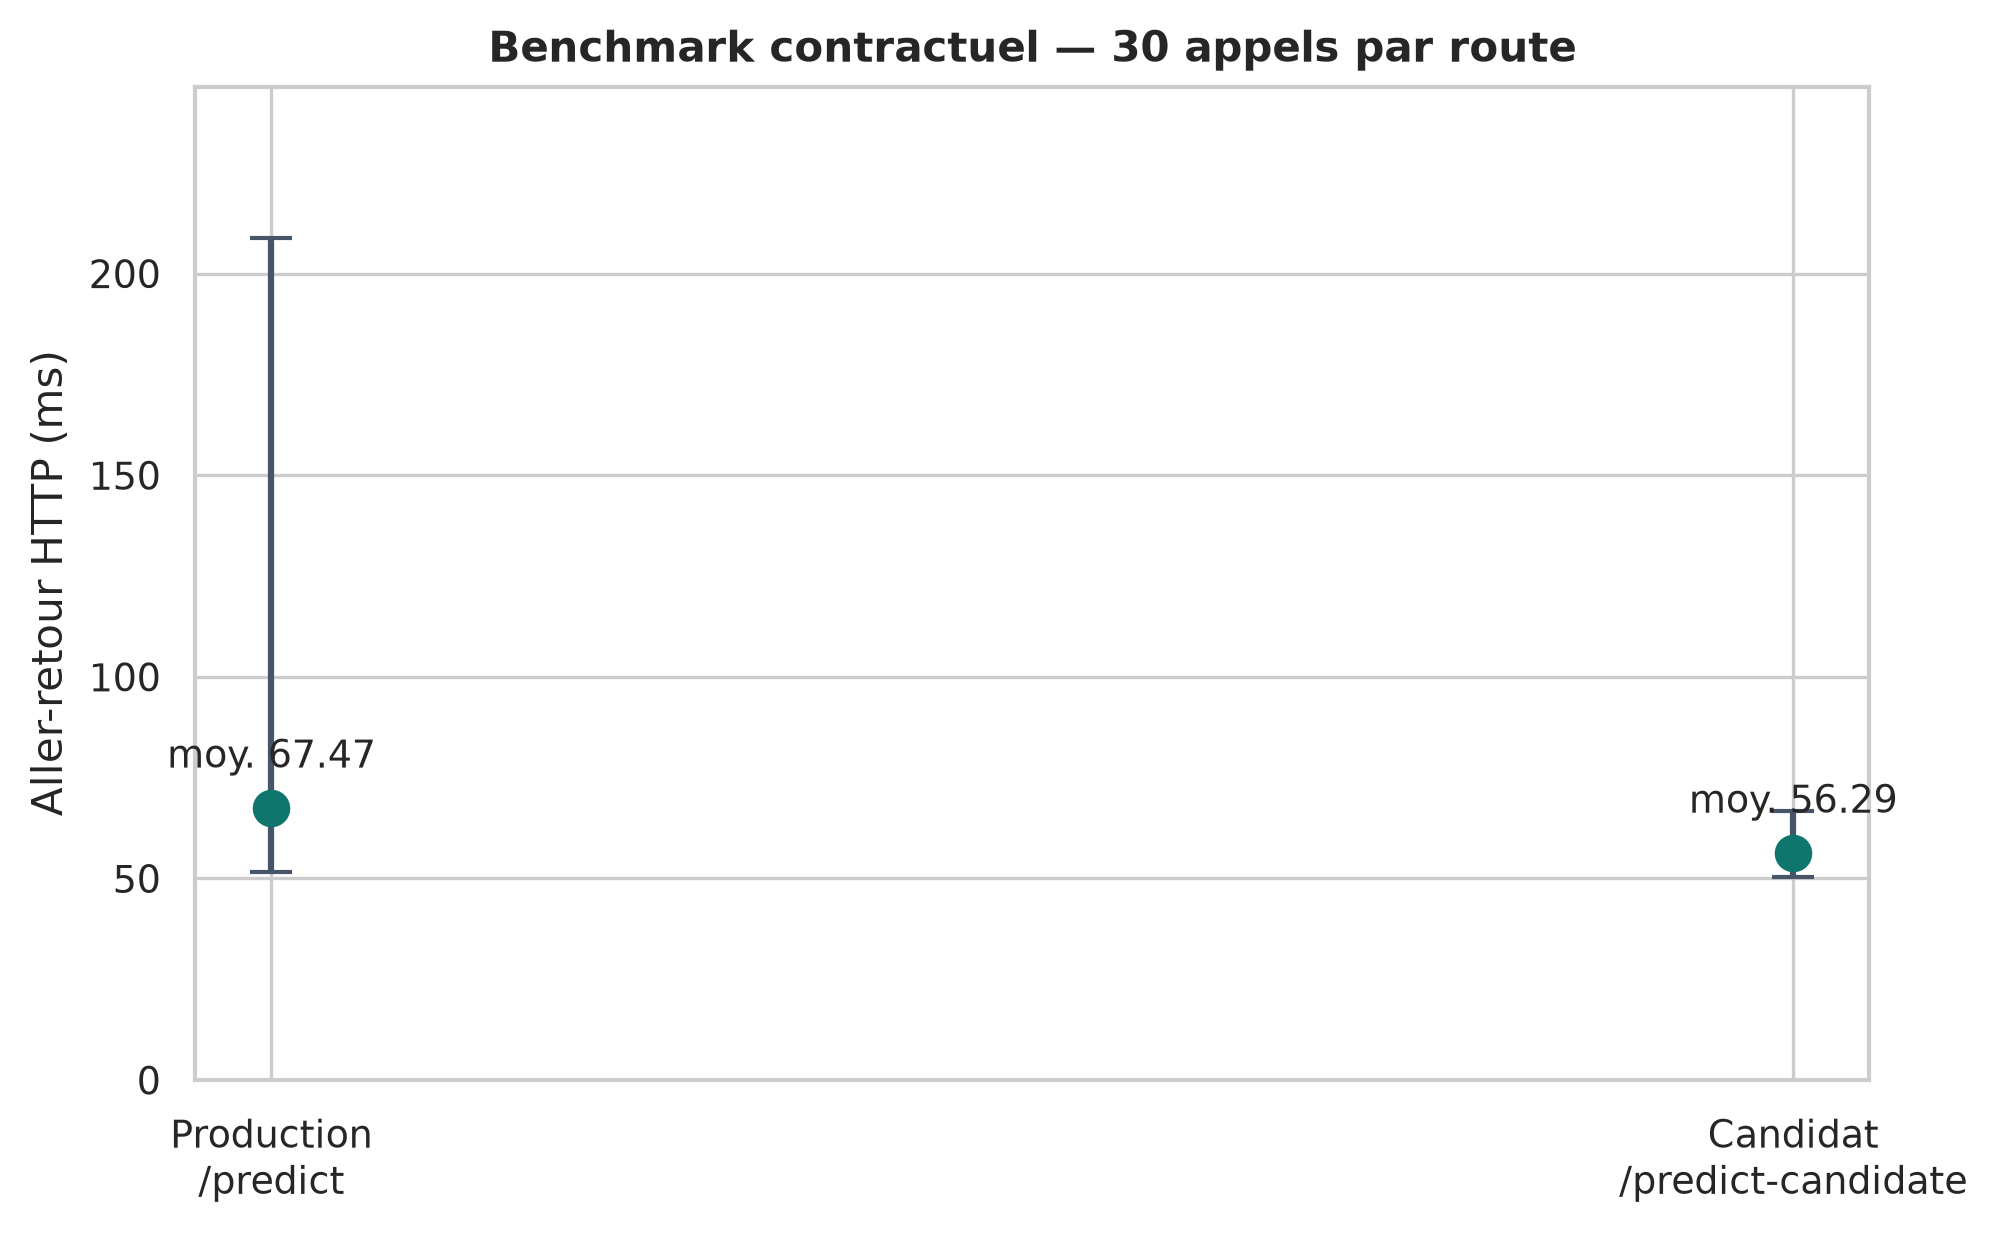
\includegraphics[width=0.94\textwidth]{figures/generated/benchmark_api_latency.png}
\caption{Latence d'aller-retour HTTP des routes de prédiction sur 30 appels contractuels.}
\label{fig:benchmark-latence}
\end{figure}

La validation ci-dessus porte sur le classifieur et l'API. Elle ne mesure pas encore le temps d'extraction MediaPipe ni la synthèse vocale. Le résultat applicatif doit donc être décrit comme une reconnaissance interactive par fenêtres, et non comme une traduction continue en temps réel.

\section{Limites et validité des conclusions}

Les résultats portent sur douze gloses isolées, des landmarks déjà extraits et un corpus contrôlé. Ils ne mesurent pas la traduction de phrases, la syntaxe LSFB, la reconnaissance de plusieurs signes successifs ni la qualité linguistique d'une sortie française.

Les performances dépendent de la qualité de MediaPipe, de l'éclairage, du cadrage, de la morphologie, de la vitesse d'exécution et des signeurs. Les cinq graines donnent une estimation utile de la variabilité, mais ne constituent pas une caractérisation exhaustive de l'incertitude. Les mesures API synthétiques ne remplacent pas un test webcam équipé et annoté.

Sur les 240 séquences isolées disponibles pour la validation exploratoire de la machine à états, une activité est détectée dans 75,4\,\% des cas et un repli ou une absence de détection est observé dans 24,6\,\% des cas. La Figure~\ref{fig:causal-detection} résume ce résultat. Les faux départs et les signes manqués ne sont pas estimables avec un corpus de signes isolés sans frontières annotées dans un flux continu ; aucune précision de segmentation ne doit donc être déduite de cette proportion.

\begin{figure}[ht]
\centering
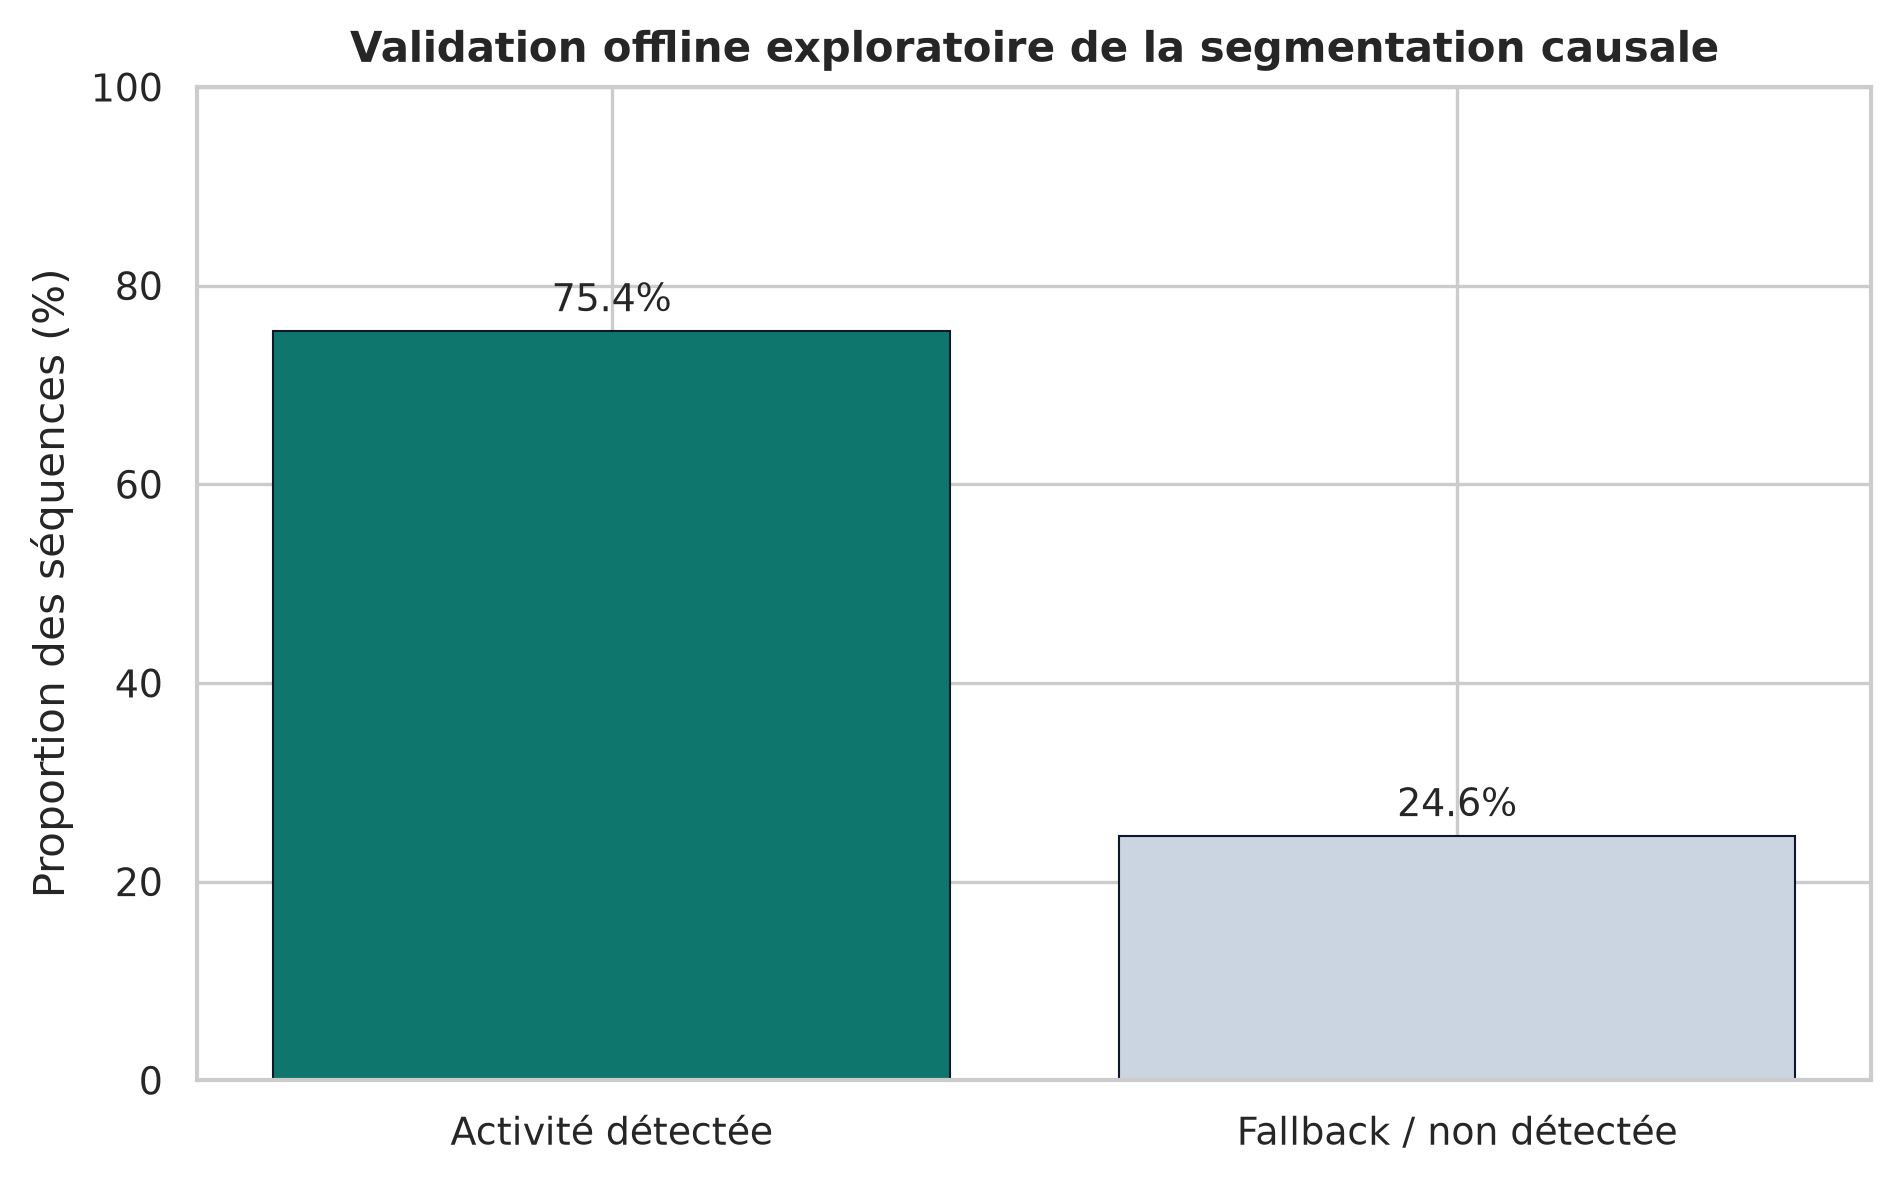
\includegraphics[width=0.94\textwidth]{figures/generated/causal_detection_offline.png}
\caption{Taux de détection de l'activité dans la validation offline exploratoire de la segmentation causale.}
\label{fig:causal-detection}
\end{figure}

La segmentation causale est une condition nécessaire pour une extension continue, mais elle ne suffit pas à transformer la reconnaissance de gloses en traduction. Une véritable traduction continue demanderait des annotations temporelles et linguistiques, une modélisation des transitions et une évaluation spécifique des phrases.

\subsection{Test de robustesse sur le split vidéo officiel}

Un test complémentaire a envoyé à l'API les 5\,957 séquences du split de test officiel. Les séquences proviennent du corpus vidéo LSFB-ISOL après extraction des landmarks autorisés ; elles ne sont donc pas des entrées synthétiques et conservent la diversité des signeurs et des gestes du test verrouillé. Chaque séquence a été rééchantillonnée sur 32 frames, transmise à \texttt{/predict-gru}, puis comparée à son étiquette de référence.

Le test API reproduit exactement les métriques de l'évaluation hors ligne. L'accuracy atteint 82,31\,\%, le macro-F1 0,8153 et la balanced accuracy 0,8129. L'écart nul avec l'audit configuration GRU retenue montre que le chargement des checkpoints, le classement top-3 et le prétraitement déployé ne dégradent pas la performance de classification.

\begin{table}[ht]
\centering
\small
\caption{Résultats détaillés de l'ensemble GRU retenu sur le test API de 5\,957 séquences.}
\label{tab:gru-api-per-class}
\begin{tabular}{lrrrr}
\hline
Glose & Précision & Rappel & F1 & Support \\
\hline
OUI & 0,8420 & 0,8993 & 0,8697 & 1\,013 \\
SOURD & 0,8047 & 0,8925 & 0,8463 & 577 \\
AVOIR & 0,8490 & 0,8224 & 0,8355 & 704 \\
QUOI & 0,8467 & 0,8571 & 0,8519 & 567 \\
REGARDER & 0,7422 & 0,8344 & 0,7856 & 483 \\
NON & 0,8097 & 0,6861 & 0,7428 & 583 \\
DIFFERENT & 0,9085 & 0,9255 & 0,9169 & 322 \\
DIRE & 0,8600 & 0,7559 & 0,8046 & 512 \\
FINIR & 0,7796 & 0,6749 & 0,7235 & 283 \\
BIEN & 0,7787 & 0,8287 & 0,8030 & 327 \\
VOIR & 0,7704 & 0,7822 & 0,7763 & 326 \\
COMPRENDRE & 0,8625 & 0,7962 & 0,8280 & 260 \\
\hline
\end{tabular}
\end{table}

Les résultats par classe montrent que DIFFERENT obtient le meilleur F1 avec 0,9169, suivi d'OUI avec 0,8697 et de QUOI avec 0,8519. Les classes les plus fragiles sont FINIR avec 0,7235 et NON avec 0,7428. La faiblesse de NON provient principalement d'un rappel de 0,6861, ce qui confirme que la confusion NON--SOURD reste une priorité d'amélioration malgré le gain global de la configuration GRU retenue.

La latence HTTP moyenne est de 63,59 millisecondes par séquence, avec une médiane de 59,57 millisecondes. Le P95 est de 86,79 millisecondes et le P99 de 109,41 millisecondes. Le maximum isolé de 758,57 millisecondes constitue une valeur atypique ; il ne doit pas être utilisé comme latence représentative sans une mesure séparée de la charge système. Ces résultats décrivent l'API et l'inférence GRU, mais n'incluent pas l'extraction MediaPipe dans le navigateur ni la synthèse vocale.

Enfin, trois payloads invalides ont été soumis pour vérifier le comportement défensif de l'API : deux formes de matrice incorrectes et un champ \texttt{landmarks} nul. Les trois requêtes ont été rejetées avec le code HTTP 422. Le test confirme donc à la fois la stabilité du modèle sur le split officiel et le respect du contrat d'entrée en cas d'erreur.

\section{Confiance, calibration et rejet}


Le modèle actif n'est pas un seul réseau. Il s'agit d'un ensemble de quinze GRU, obtenu avec trois graines et cinq folds. Pour une séquence, chaque réseau produit un vecteur de douze valeurs réelles avant normalisation. Ces valeurs sont appelées \emph{logits}. Un logit n'est pas une probabilité : il peut être positif ou négatif et mesure seulement la préférence relative du réseau pour une classe.

Chaque vecteur de logits $z^{(m)}$ est converti en distribution par la fonction softmax :
\[
p^{(m)}_c=\frac{\exp(z^{(m)}_c)}{\sum_{j=1}^{C}\exp(z^{(m)}_j)},
\qquad C=12.
\]
Les valeurs $p^{(m)}_c$ sont positives et leur somme vaut un. L'application calcule ensuite la moyenne des quinze distributions :
\[
\bar p_c=\frac{1}{15}\sum_{m=1}^{15}p^{(m)}_c.
\]
La classe affichée est $\hat y=\arg\max_c\bar p_c$. Dans la version actuelle non calibrée, le champ \texttt{confidence} est exactement $\max_c\bar p_c$. Par exemple, si la moyenne donne 0,77 pour OUI, 0,09 pour NON et 0,05 pour COMPRENDRE, l'application affiche OUI avec un score de 0,77. Ce score décrit la préférence probabiliste interne de l'ensemble ; il ne signifie pas encore que 77\,\% des séquences affichées avec ce score sont correctes.

Cette distinction est importante. Les quinze réseaux sont plusieurs entraînements du même type de GRU, et non quinze architectures différentes. Leur diversité vient des graines et des partitions de validation. L'accord de l'ensemble est mesuré séparément par la proportion de réseaux dont la classe top-1 est la classe finale :
\[
\mathrm{Accord}=\frac{1}{15}\sum_{m=1}^{15}\mathbf{1}\!\left(\arg\max_c p^{(m)}_c=\hat y\right).
\]
La marge entre les deux meilleures classes complète ce diagnostic :
\[
\mathrm{Marge}=\bar p_{(1)}-\bar p_{(2)}.
\]

La calibration vise à rapprocher le score affiché de la fréquence réelle de correction. La méthode retenue pour le prototype est la \emph{temperature scaling}. Elle introduit une température positive $T$ avant softmax :
\[
p_{T,c}=\frac{\exp(z_c/T)}{\sum_{j=1}^{C}\exp(z_j/T)}.
\]
Lorsque $T>1$, la distribution est aplatie et les scores trop confiants diminuent. Lorsque $T<1$, elle devient plus concentrée. La valeur $T$ doit être apprise en minimisant la log-vraisemblance négative sur des prédictions hors-échantillon de validation groupée par signeur. Le test officiel ne doit jamais servir à apprendre $T$ ou les seuils de rejet.

Dans l'implémentation actuelle, les sorties probabilistes des quinze réseaux sont d'abord moyennées, puis la température est appliquée à cette distribution agrégée. Le champ \texttt{raw\_confidence} conserve le maximum avant calibration et le champ \texttt{confidence} contient le maximum après calibration lorsqu'un artefact de calibration est présent. Tant que les probabilités hors-échantillon nécessaires ne sont pas archivées, l'API conserve \texttt{confidence\_calibrated=false} et \texttt{accepted=null} ; elle n'invente donc ni température ni seuil à partir du test officiel.

Le rejet est une décision séparée du classement. Il ne change pas la classe top-1 ; il décide seulement si cette classe peut être présentée comme suffisamment fiable. La règle future combinera la confiance calibrée, la marge et l'accord des quinze réseaux :
\[
\mathrm{accept}=\left(\mathrm{confidence}\geq\tau_c\right)\land\left(\mathrm{marge}\geq\tau_m\right)\land\left(\mathrm{accord}\geq\tau_a\right).
\]
Les seuils seront choisis sur validation selon un objectif de couverture fixé à l'avance, par exemple au moins 85\,\% des séquences. Le critère rapporté sera le couple couverture--risque : la couverture est la proportion de séquences acceptées et le risque est le taux d'erreur parmi ces séquences. Un seuil ne sera pas retenu parce qu'il paraît intuitif ; il devra être inscrit avant l'évaluation finale et accompagné d'un intervalle d'incertitude obtenu par bootstrap groupé par signeur.

Pour l'utilisateur, trois états sont préférables à un rejet systématique. Une décision calibrée et séparée est affichée directement. Une décision intermédiaire conserve le top-1 et le top-3, mais désactive la vocalisation automatique. Une décision rejetée demande une nouvelle capture et indique que la capture est incertaine. Cette politique réduit le risque d'afficher une classe fausse comme certaine sans supprimer inutilement les réponses utiles.


\section{Conclusion du chapitre}
L'évaluation récente montre que l'ensemble GRU retenu constitue le meilleur résultat observé, avec un macro-F1 de 0,8153, tandis que le Random Forest complet atteint 0,7839. Le test de robustesse sur les 5\,957 séquences via l'API reproduit exactement ces métriques. La GRU est donc le modèle actif de l'application, tandis que le RF reste conservé comme référence de comparaison et solution de retour arrière.

La calibration isotonic améliore fortement la fiabilité des scores RF, mais ne doit pas être confondue avec une amélioration de la classification. Les anciennes baselines sont utiles pour documenter la progression, mais les conclusions principales du mémoire reposent désormais sur GRU initiale, configuration GRU retenue, Random Forest complet et le test de robustesse API. La prochaine étape est une comparaison à représentation identique, suivie d'une mesure complète de la chaîne webcam et d'une politique de rejet calibrée.

Cette conclusion est une conclusion de reconnaissance contrôlée, pas une preuve de traduction ouverte ni de temps réel strict. Le test API porte sur des landmarks extraits de séquences vidéo et ne mesure pas encore le coût MediaPipe ni la synthèse vocale. La prochaine étape scientifique est donc la validation de la chaîne complète sur des flux webcam réels.
